\documentclass[t]{beamer}
\usepackage{media9}
\usepackage{graphicx}
\mode<presentation> {
  \usetheme{boxes}
  \usecolortheme{rose}
  \setbeamertemplate{navigation symbols}{} % To remove the navigation symbols from the bottom of all slides uncomment this line
}

%\usepackage{pgfpages}
%\pgfpagesuselayout{2 on 1}[a4paper,border shrink=5mm]

\usefonttheme[onlymath]{serif}
\usepackage{fontspec} 
\defaultfontfeatures{Mapping=tex-text} 
\setsansfont[Ligatures={Common}]{Futura}
\setmonofont[Scale=0.8]{Monaco} 

\usepackage{graphicx} % Allows including images
\usepackage{booktabs} % Allows the use of \toprule, \midrule and \bottomrule in tables

%----------------------------------------------------------------------------------------
% New Commands
%----------------------------------------------------------------------------------------

\newcommand*{\movie}[1]{\includemedia[width=0.6\linewidth,height=0.3375\linewidth, activate=pageopen]{}{#1}}
\newcommand{\img}[1]{\includegraphics[width=1\linewidth]{images/#1}}
\newcommand{\imgs}[1]{\includegraphics[width=.75\linewidth]{images/#1}}
\newcommand{\imgss}[1]{\includegraphics[width=.5\linewidth]{images/#1}}
\newcommand{\bi}{\begin{itemize}}
\newcommand{\ei}{\end{itemize}}

%----------------------------------------------------------------------------------------
%	TITLE PAGE
%----------------------------------------------------------------------------------------
\title[Topic 2]{Grade 8: Light and Optics} % The short title appears at the bottom of every slide, the full title is only on the title page
\subtitle{Topic 2: Reflections}
\author{Dr. Pineda} 
\institute[] {\href{http://www.drpineda.ca}{www.drpineda.ca}}
\date{} % Date, can be changed to a custom date

% Customize the footline
%\setbeamertemplate{footline}{goo \insertframenumber \insertsubtitle \inserttitle}

\setbeamertemplate{footline}{
   \begin{beamercolorbox}[ht=4ex,leftskip=.2cm,rightskip=.2cm]{author in head/foot}
    \usebeamercolor{UniBlue}
    \hrule
    \vspace{0.1cm}
    \inserttitle \ - \insertsubtitle \hfill \insertframenumber/\inserttotalframenumber
   \end{beamercolorbox}
   \vspace*{0.1cm}
} 

%----------------------------------------------------------------------------------------
%	BEGIN DOCUMENT
%----------------------------------------------------------------------------------------
\begin{document}

{
\setbeamertemplate{footline}{} % no page number here
\frame{\titlepage}
}

%----------------------------------------------------------------------------------------
%	PRESENTATION SLIDES
%----------------------------------------------------------------------------------------

%----------------------------------------------------------------------------------------
%	Reflection
%----------------------------------------------------------------------------------------
\begin{frame}{Reflection}
Process in which light strikes a surface and bounces back off that surface. 
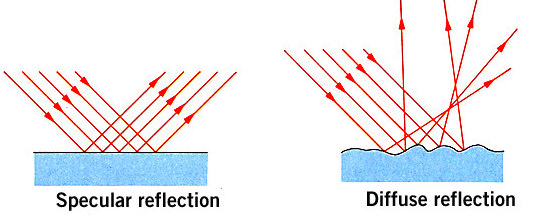
\includegraphics[width=1\linewidth]{images/specularreflection.jpg}
\end{frame}

%----------------------------------------------------------------------------------------
%	Specular vs. Diffuse Reflection
%----------------------------------------------------------------------------------------
\begin{frame}{Specular vs. Diffuse Reflection}

\begin{description}
\item[Specular reflection:]  Mirror-like reflection of light from a surface, in which light from a single incoming direction (a ray) is reflected into a single outgoing direction. A smooth surface will have all light reflect together and form a clear image

\item[Diffuse reflection:]  Reflection of light from a surface such that an incident ray is reflected at many angles rather than at just one angle as in the case of specular reflection. A rough surface will scatter light and will not form a clear image
\end{description}
\end{frame}

%----------------------------------------------------------------------------------------
%	Scientific Law
%----------------------------------------------------------------------------------------
\begin{frame}{Scientific Law}
\bi
\item A scientific law is a statement of a pattern that has been observed and tested again and again with the same results each time. \item Scientific laws \underline{do not explain why} we see a pattern.
\ei
\img{law-of-gravity-enforced.jpg}
\end{frame}

%----------------------------------------------------------------------------------------
%	Law of Reflection
%----------------------------------------------------------------------------------------
\begin{frame}{Law of Reflection}
\bi
\item Angle of incidence equals the angle of reflection
\item The incident and reflected rays and the normal are all on the same plane
\ei
\img{law_of_reflection.png}
\end{frame}

%----------------------------------------------------------------------------------------
%	How do we see reflections?
%----------------------------------------------------------------------------------------
\begin{frame}{How do we see reflections?}
\imgs{mirror.jpg}
\end{frame}

%----------------------------------------------------------------------------------------
%	How do we see reflections?
%----------------------------------------------------------------------------------------
\begin{frame}{How do we see reflections?}
The distance between object and plane (mirror surface) is same as distance between plane and virtual image.
\end{frame}

%----------------------------------------------------------------------------------------
%	Concave vs. Convex Surfaces
%----------------------------------------------------------------------------------------
\begin{frame}{Concave vs. Convex Surfaces}
\begin{description}
\item[Concave:] \only<beamer>{The surface "caves" inwards}
\item[Convex:] \only<beamer>{The surface pushes or bulges outwards}
\end{description}
\imgs{spoon.jpg}
\end{frame}

\begin{frame}[allowframebreaks]
\frametitle{Paragraphs of Text}
Sed iaculis dapibus gravida. Morbi sed tortor erat, nec interdum arcu. Sed id lorem lectus. Quisque viverra augue id sem ornare non aliquam nibh tristique. Aenean in ligula nisl. Nulla sed tellus ipsum. Donec vestibulum ligula non lorem vulputate fermentum accumsan neque mollis.\\~\\

Sed diam enim, sagittis nec condimentum sit amet, ullamcorper sit amet libero. Aliquam vel dui orci, a porta odio. Nullam id suscipit ipsum. Aenean lobortis commodo sem, ut commodo leo gravida vitae. Pellentesque vehicula ante iaculis arcu pretium rutrum eget sit amet purus. Integer ornare nulla quis neque ultrices lobortis. Vestibulum ultrices tincidunt libero, quis commodo erat ullamcorper id.\~\

Sed iaculis dapibus gravida. Morbi sed tortor erat, nec interdum arcu. Sed id lorem lectus. Quisque viverra augue id sem ornare non aliquam nibh tristique. Aenean in ligula nisl. Nulla sed tellus ipsum. Donec vestibulum ligula non lorem vulputate fermentum accumsan neque mollis.\\~\\

Sed diam enim, sagittis nec condimentum sit amet, ullamcorper sit amet libero. Aliquam vel dui orci, a porta odio. Nullam id suscipit ipsum. Aenean lobortis commodo sem, ut commodo leo gravida vitae. Pellentesque vehicula ante iaculis arcu pretium rutrum eget sit amet purus. Integer ornare nulla quis neque ultrices lobortis. Vestibulum ultrices tincidunt libero, quis commodo erat ullamcorper id.

\end{frame}

%------------------------------------------------

\begin{frame}[shrink]
\frametitle{Math}
\[
x = \frac{1}{\pi}
\]
\end{frame}

%------------------------------------------------

\begin{frame}<handout:0>
\frametitle{Bullet Points}
\begin{itemize}
\item Lorem ipsum dolor sit amet, consectetur adipiscing elit
\item Aliquam blandit faucibus nisi, sit amet dapibus enim tempus eu
\item Nulla commodo, erat quis gravida posuere, elit lacus lobortis est, quis porttitor odio mauris at libero
\item Nam cursus est eget velit posuere pellentesque
\item Vestibulum faucibus velit a augue condimentum quis convallis nulla gravida
\end{itemize}
\end{frame}

%------------------------------------------------

\begin{frame}
\frametitle{Blocks of Highlighted Text}
\begin{block}{Block 1}
Lorem ipsum dolor sit amet, consectetur adipiscing elit. Integer lectus nisl, ultricies in feugiat rutrum, porttitor sit amet augue. Aliquam ut tortor mauris. Sed volutpat ante purus, quis accumsan dolor.
\end{block}

\begin{block}{Block 2}
Pellentesque sed tellus purus. Class aptent taciti sociosqu ad litora torquent per conubia nostra, per inceptos himenaeos. Vestibulum quis magna at risus dictum tempor eu vitae velit.
\end{block}

\begin{block}{Block 3}
Suspendisse tincidunt sagittis gravida. Curabitur condimentum, enim sed venenatis rutrum, ipsum neque consectetur orci, sed blandit justo nisi ac lacus.
\end{block}
\end{frame}

%------------------------------------------------


\begin{frame}
 
   \begin{block}{This is a Block}
      This is important information
   \end{block}
 
   \begin{alertblock}{This is an Alert block}
   This is an important alert
   \end{alertblock}
 
   \begin{exampleblock}{This is an Example block}
   This is an example 
   \end{exampleblock}
 
\end{frame}

%------------------------------------------------

\begin{frame}
\frametitle{Multiple Columns}
\begin{columns}[c] % The "c" option specifies centered vertical alignment while the "t" option is used for top vertical alignment

\column{.45\textwidth} % Left column and width
\textbf{Heading}
\begin{enumerate}
\item Statement
\item Explanation
\item Example
\end{enumerate}

\column{.5\textwidth} % Right column and width
Lorem ipsum dolor sit amet, consectetur adipiscing elit. Integer lectus nisl, ultricies in feugiat rutrum, porttitor sit amet augue. Aliquam ut tortor mauris. Sed volutpat ante purus, quis accumsan dolor.

\end{columns}
\end{frame}

%------------------------------------------------
\section{Second Section}
%------------------------------------------------

\begin{frame}
\frametitle{Table}
\begin{table}
\begin{tabular}{l l l}
\toprule
\textbf{Treatments} & \textbf{Response 1} & \textbf{Response 2}\\
\midrule
Treatment 1 & 0.0003262 & 0.562 \\
Treatment 2 & 0.0015681 & 0.910 \\
Treatment 3 & 0.0009271 & 0.296 \\
\bottomrule
\end{tabular}
\caption{Table caption}
\end{table}
\end{frame}

%------------------------------------------------

\begin{frame}
\frametitle{Theorem}
\begin{theorem}[Mass--energy equivalence]
$E = mc^2$
\end{theorem}
\end{frame}

%------------------------------------------------

\begin{frame}[fragile] % Need to use the fragile option when verbatim is used in the slide
\frametitle{Verbatim}
\begin{example}[Theorem Slide Code]
\begin{verbatim}
\begin{frame}
\frametitle{Theorem}
\begin{theorem}[Mass--energy equivalence]
$E = mc^2$
\end{theorem}
\end{frame}\end{verbatim}
\end{example}
\end{frame}

%------------------------------------------------

\begin{frame}
\frametitle{Figure}
Uncomment the code on this slide to include your own image from the same directory as the template .TeX file.
%\begin{figure}
%\includegraphics[width=0.8\linewidth]{test}
%\end{figure}
\end{frame}

%------------------------------------------------

\begin{frame}[fragile] % Need to use the fragile option when verbatim is used in the slide
\frametitle{Citation}
An example of the \verb|\cite| command to cite within the presentation:\\~

This statement requires citation \cite{p1}.
\end{frame}

%------------------------------------------------

\begin{frame}
\frametitle{References}
\footnotesize{
\begin{thebibliography}{99} % Beamer does not support BibTeX so references must be inserted manually as below
\bibitem[Smith, 2012]{p1} John Smith (2012)
\newblock Title of the publication
\newblock \emph{Journal Name} 12(3), 45 -- 678.
\end{thebibliography}
}
\end{frame}

\end{document}